\documentclass[12pt,a4paper]{book}
\usepackage[utf8]{inputenc}
\usepackage[T1]{fontenc}
\usepackage[italian]{babel}
\usepackage{amsmath}
\usepackage{amsfonts}
\usepackage{amssymb}
\usepackage{graphicx}
\usepackage{import}

\usepackage{cite}

\usepackage{todonotes}

\newcommand{\Fig}[0]{Fig.}

%inserire gestione figura

\title{Progetto di un sistema optoelettronico indossabile per misure fotopletismografiche}
\author{Wasim Esbai, Matteo Verzeroli}

\pagestyle{plain}

\begin{document}
	\maketitle
	
	\tableofcontents
	
	\chapter*{Introduzione}
	\addcontentsline{toc}{chapter}{Introduzione}
	
	Example of a Figure
	\todo{Example of a figure}
	\begin{figure}[h]
		\centering
		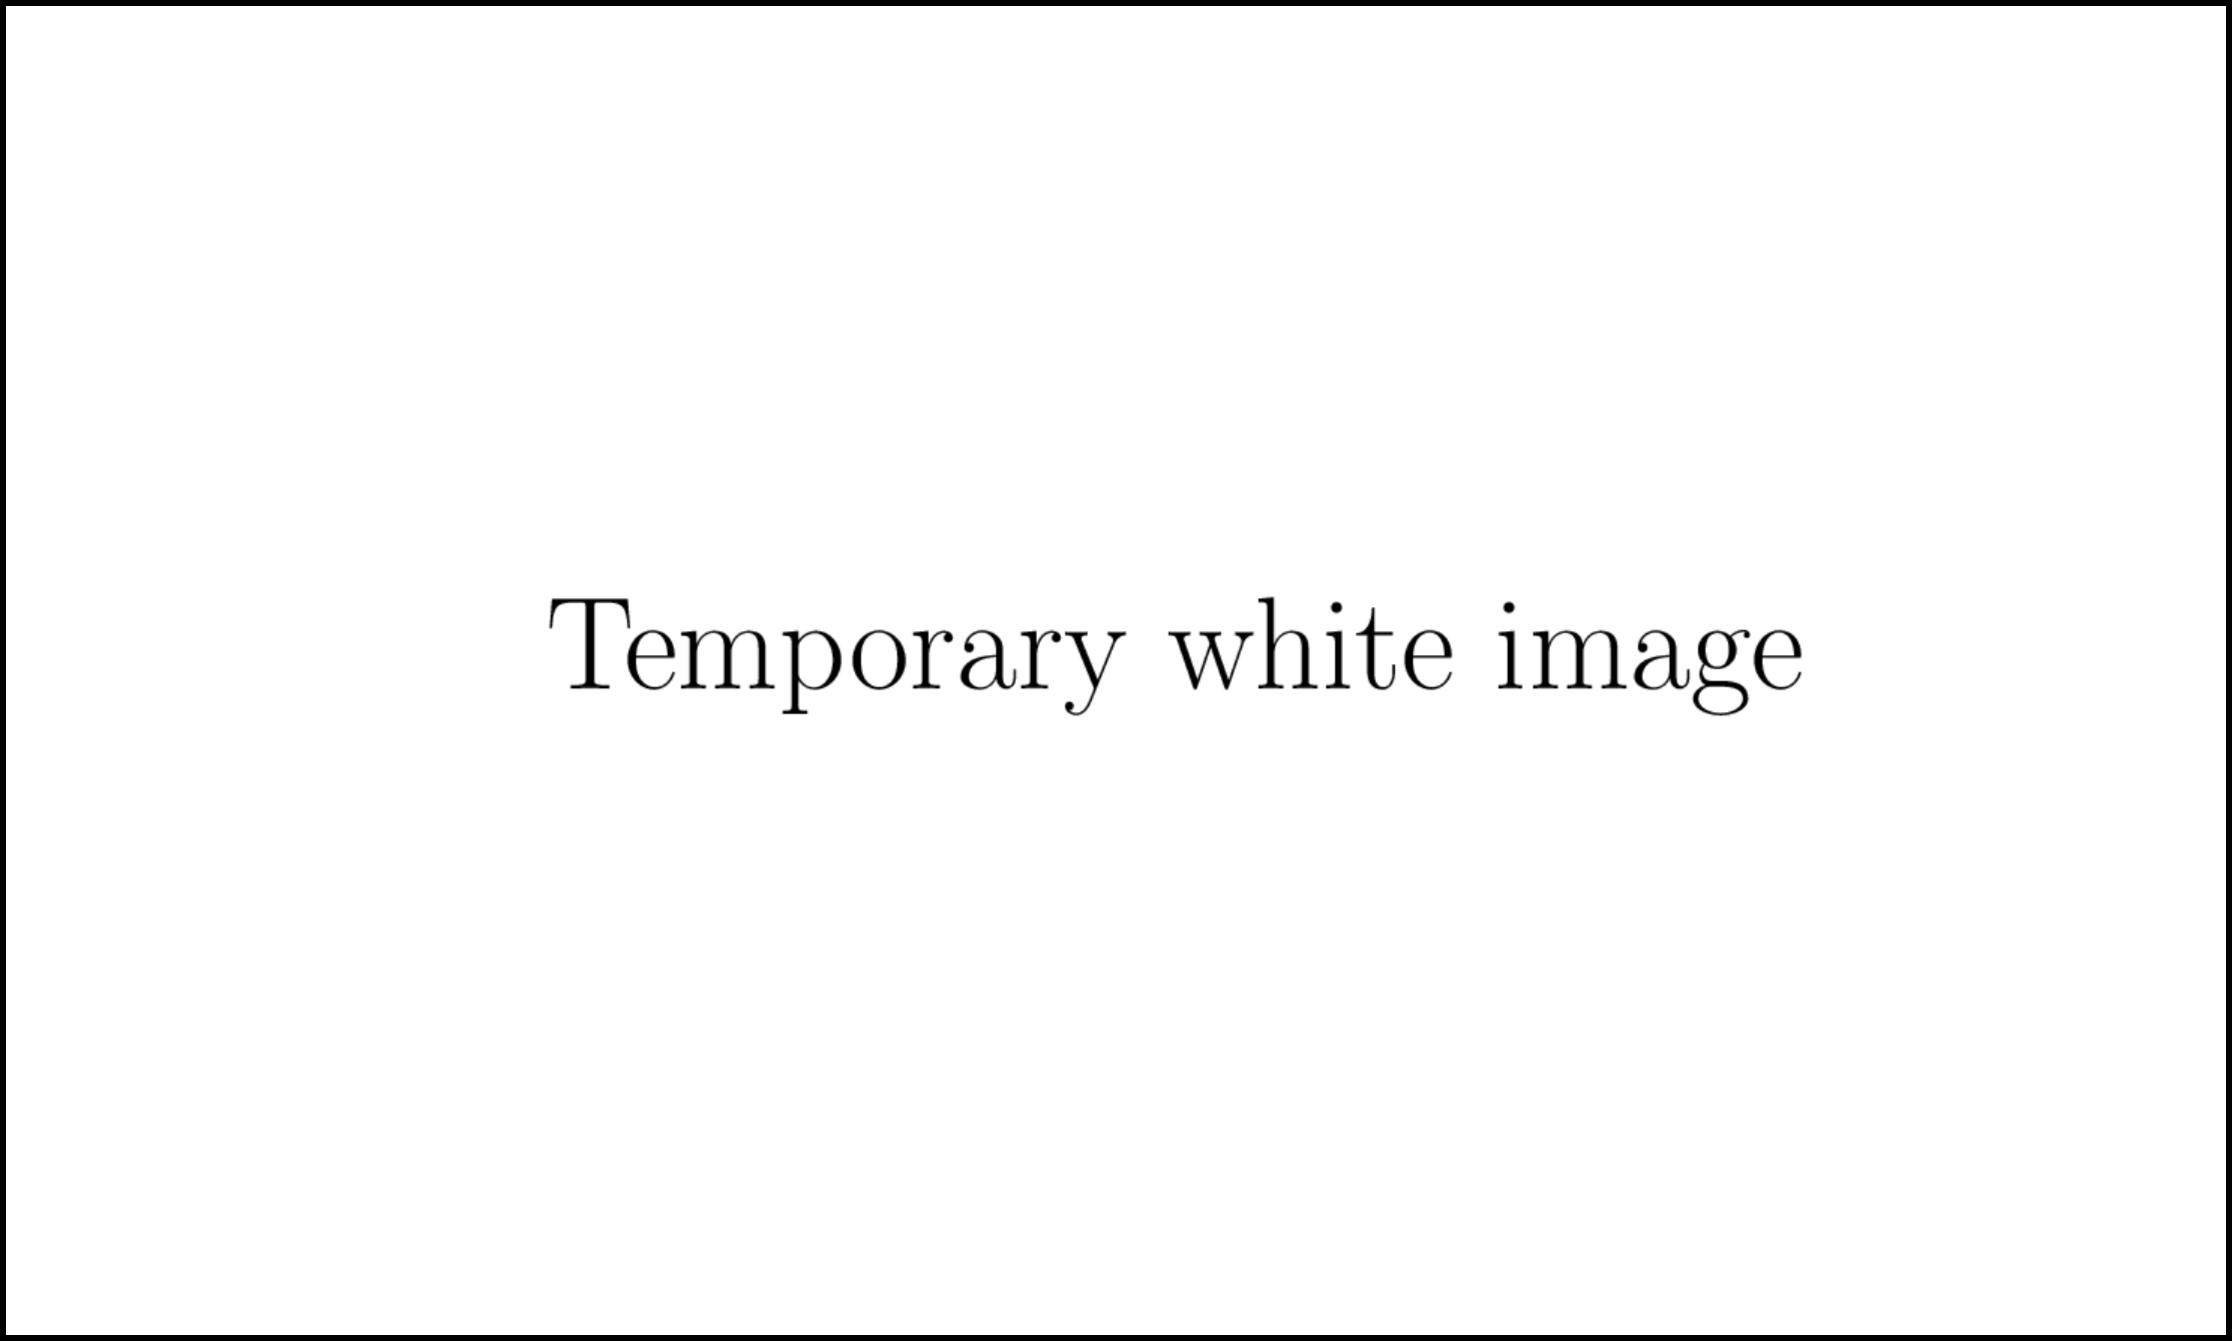
\includegraphics[width=0.7\linewidth]{ImageFiles/Fotopletismografia/white_img}
		\caption{xx}
		\label{fig:xx}
	\end{figure}
	
	Relying on the \Fig~\ref{fig:xx},
	
	\chapter{Fotopletismografia}
	\import{./TextFiles/Fotopletismografia/}{Principio di funzionamento.tex}
	\import{./TextFiles/Fotopletismografia/}{Siti di misura e lunghezze d’onda impiegate.tex}
	\import{./TextFiles/Fotopletismografia/}{Stato dell’arte dei moduli PPG.tex}
	
	\chapter{Progetto della piattaforma indossabile}
	\import{./TextFiles/Progetto della piattaforma indossabile/}{Hardware dell’adapter board.tex}
	\import{./TextFiles/Progetto della piattaforma indossabile/}{Firmware.tex}
	
	\chapter{Caratterizzazione della piattaforma indossabile}
	\import{./TextFiles/Caratterizzazione della piattaforma indossabile/}{Consumo di potenza.tex}
	\import{./TextFiles/Caratterizzazione della piattaforma indossabile/}{Sito di misura.tex}
	
	\chapter*{Conclusioni}
	\addcontentsline{toc}{chapter}{Conclusioni}
	
	\bibliographystyle{plain}
	\bibliography{./OtherFiles/bibliography}
	\addcontentsline{toc}{chapter}{Bibliografia}

	
	
\end{document}